%--------------------------------------------------------------------%
% Page          : Chapter 3 - Metodologi (Methodology)
%--------------------------------------------------------------------%

\chapter{METODOLOGI}
\label{sec:metodologi}

Bab ini menjelaskan mengenai metodologi yang digunakan untuk menjawab rumusan masalah beserta tujuan penelitian yang dipaparkan sebelumnya. Adapun secara garis besar metodologi penelitian yang digunakan peneliti diilustrasikan seperti pada Gambar~\ref{fig:alur-penelitian}.

\begin{figure}[htbp]
    \centering
    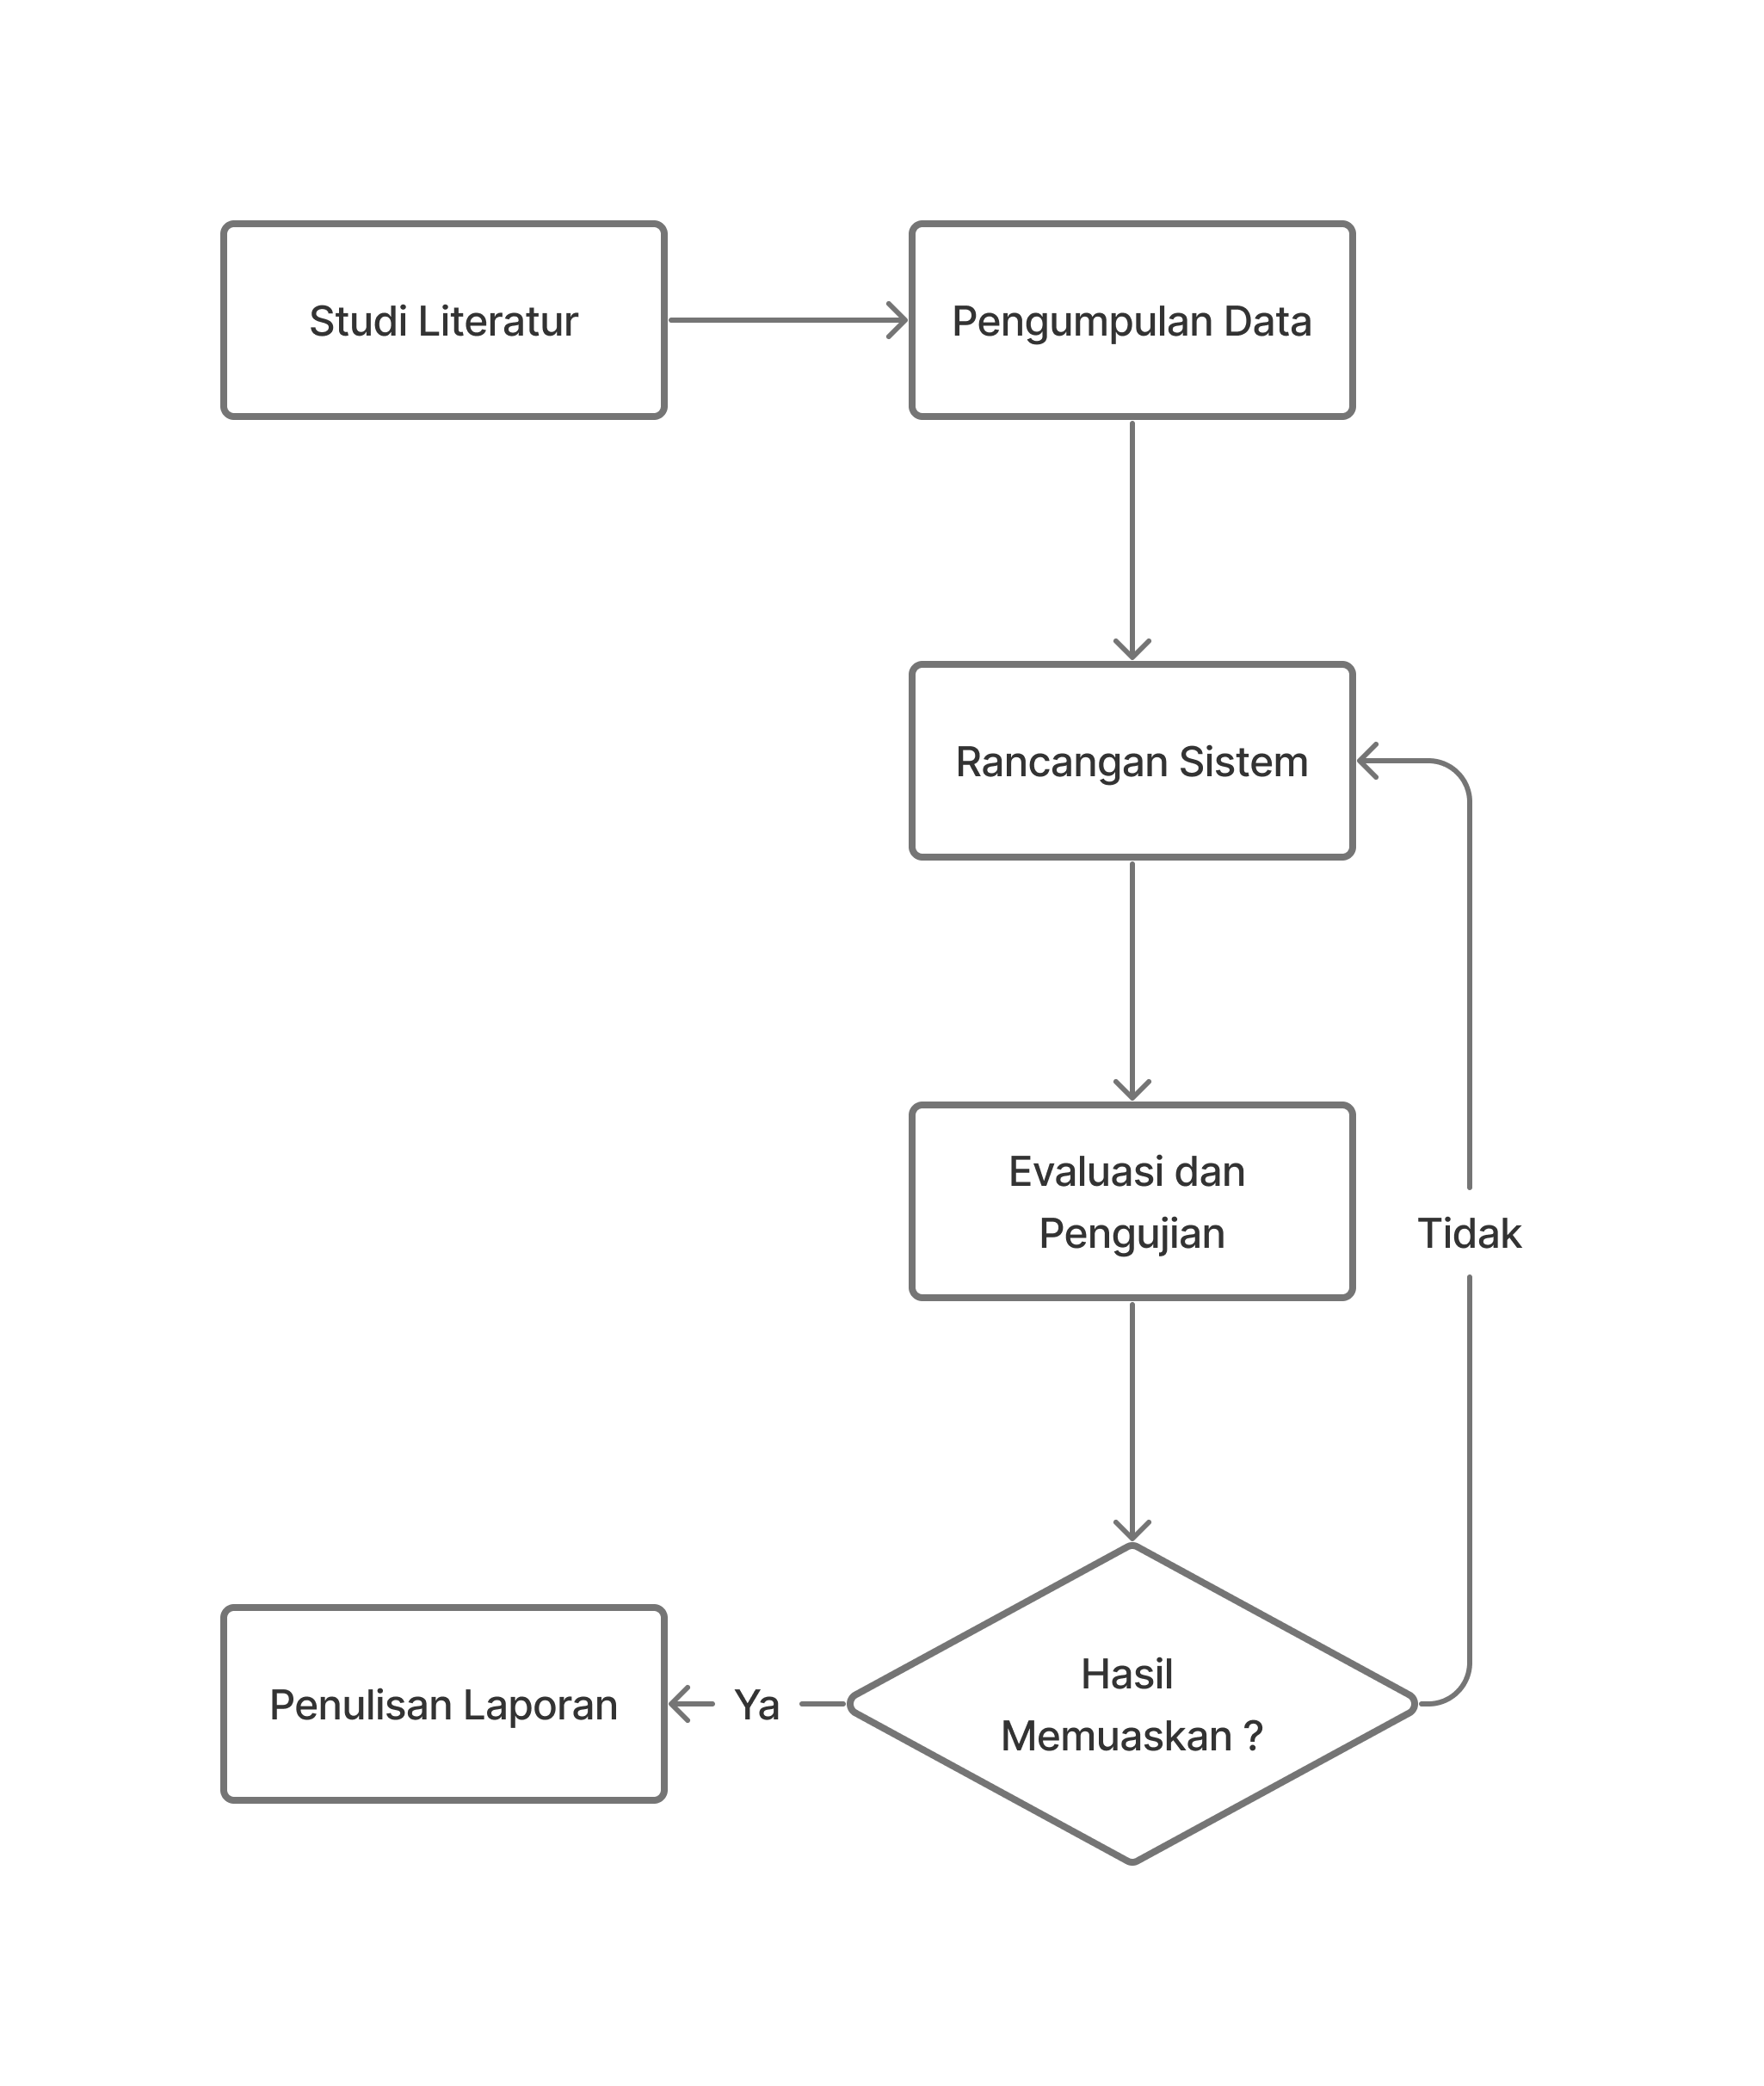
\includegraphics[keepaspectratio, width=0.6\textwidth]{src/resources/figures/image11.png}
    \caption{Alur penelitian tesis}
    \label{fig:alur-penelitian}
\end{figure}

Penelitian ini terdiri dari beberapa tahapan yang terdiri dari 1) studi literatur, 2) pengumpulan data, 3) rancangan sistem, 4) pengujian, 5) analisis hasil, dan 6) penulisan laporan. Setiap tahapan metodologi penelitian ini akan dijelaskan dengan lebih rinci pada setiap subbab.

\section{Studi Literatur}
\label{sec:studi-literatur}

Studi literatur merupakan tahapan awal dalam penelitian ini. Studi literatur dilakukan untuk mencari referensi dari berbagai sumber mengenai penelitian yang terkait dan memiliki kemiripan dengan penelitian yang dilakukan. Studi literatur juga perlu dilakukan agar bisa memahami metode dan konsep sesuai pembahasan dan permasalahan yang akan diselesaikan sehingga bisa memberi solusi. Adapun literatur utama terkait dengan metode \emph{scalling} pada Kubernetes dan Serverless mengacu pada penelitian yang dilakukan oleh \citet{senjab2023survey}, dan \citet{mampage2022holistic}. Sedangkan untuk algoritma \emph{Elax} yang akan dijadikan dasar metode untuk dimodifikasi mengacu pada penelitian \citet{yang2019elax}. Salah satu modifikasi yang dilakukan adalah mengganti bagian \emph{load predictor} dari LSTM menjadi GRU.

\section{Pengumpulan Data}
\label{sec:pengumpulan-data}

Pada tahapan ini, dilakukan pengumpulan data untuk \emph{training} prediktor beban \emph{traffic} dan simulasi \emph{load testing} pada aplikasi. Data \emph{training} digunakan untuk melatih prediktor time-series berbasis GRU. Adapun data yang akan digunakan pada penelitian ini adalah data traffic load pada ClarkNet dan Calgary trace. Struktur data terdiri dari:

\begin{enumerate}
    \item \textbf{host} yang meminta request. Dapat berupa nama host, atau IP address.
    \item \textbf{Timestamp} dalam format ``DAY MON DD HH:MM:SS YYYY'', dimana:
    \begin{enumerate}
        \item DAY: hari dalam pekan
        \item MON: nama bulan
        \item DD: tanggal dalam bulan
        \item HH:MM:SS: waktu pada hari dengan format 24 jam
        \item YYYY: tahun
    \end{enumerate}
    \item \textbf{request} metode dan URL request untuk HTTP protocol
    \item \textbf{HTTP} reply code
    \item \textbf{Bytes}: Ukuran bytes dalam reply
\end{enumerate}

Data merupakan log seluruh request HTTP ke ClarkNet WWW dan University of Calgary's Department of Computer Science, dengan total data 4.055.326 \emph{requests}. Berikut contoh sampel data request yang digunakan pada Tabel~\ref{tab:dataset-request}.

\begin{table}[htbp]
    \centering
    \caption{Contoh dataset request}
    \label{tab:dataset-request}
    \small
    \begin{tabular}{p{0.3\textwidth} p{0.6\textwidth}}
        \toprule
        \textbf{Dataset} & \textbf{Request} \\
        \midrule
        University of Calgary's Department of Computer Science & \texttt{local - - [24/Oct/1994:13:41:41 -0600] "GET index.html HTTP/1.0" 200 150} \\
        & \texttt{local - - [24/Oct/1994:13:41:41 -0600] "GET 1.gif HTTP/1.0" 200 1210} \\
        & \texttt{local - - [24/Oct/1994:13:43:13 -0600] "GET index.html HTTP/1.0" 200 3185} \\
        \midrule
        ClarkNet & \texttt{204.249.225.59 - - [28/Aug/1995:00:00:34 -0400] "GET /pub/rmharris/catalogs/dawsocat/intro.html HTTP/1.0" 200 3542} \\
        & \texttt{access9.accsyst.com - - [28/Aug/1995:00:00:35 -0400] "GET /pub/robert/past99.gif HTTP/1.0" 200 4993} \\
        & \texttt{access9.accsyst.com - - [28/Aug/1995:00:00:35 -0400] "GET /pub/robert/curr99.gif HTTP/1.0" 200 5836} \\
        \bottomrule
    \end{tabular}
\end{table}

\section{Perancangan Metode}
\label{sec:perancangan-metode}

Proses ini menjelaskan tentang perancangan metode yang akan diajukan untuk melakukan \emph{routing} antara kluster dan \emph{scalling alokasi} sumber daya, berdasarkan hasil prediksi permintaan di masa mendatang dan kondisi \emph{tail latency} saat ini.

\section{Implementasi Metode}
\label{sec:implementasi-metode}

Bagian ini menjelaskan implementasi dari rancangan metode yang akan dikerjakan dari rangkaian penelitian ini. Tujuan akhir dari penelitian ini adalah membangun metode \emph{scalling} dan \emph{routing traffic dinamis} yang mengintegrasikan Kubernetes dan Serverless. Metode yang diusulkan terdiri dari 3 bagian:

\subsection{Load Predictor}
\label{sec:load-predictor}

Load Predictor berfungsi untuk memperkirakan lalu lintas jaringan di masa mendatang berdasarkan data historis. Berikut adalah langkah-langkah implementasi:

\begin{enumerate}
    \item \textbf{Pemrosesan Data}
\end{enumerate}

Data historis yang digunakan dijelaskan pada bagian \ref{sec:pengumpulan-data}. Data tersebut kemudian ditransformasikan menjadi bentuk \emph{Request Per-Second} (RPS) untuk mendapatkan volume traffic jaringan. GRU dipilih karena lebih efisien dalam hal penggunaan sumber daya dan waktu pelatihan \citep{mondal2023toward}.

\begin{enumerate}
    \setcounter{enumi}{1}
    \item \textbf{Struktur Model}
\end{enumerate}

Model menggunakan konfigurasi \emph{multi-point prediction} karena terdapat cost ketika rekonfigurasi cluster sehingga konfigurasi tidak dapat dilakukan terlalu sering. Jumlah data point yang akan diprediksi adalah 30 detik ke depan.

\subsection{Resource Alocator}
\label{sec:resource-alocator}

Blok ini berfungsi untuk menghitung jumlah sumber daya yang harus disiapkan terhadap volume permintaan yang akan diterima selama 30 detik ke depan. Untuk memodelkan kebutuhan sumber daya, digunakan model persamaan linear:

\begin{equation}
    R = \alpha \cdot x + \beta
    \label{eq:resource-model}
\end{equation}

dimana $R$ menunjukkan jumlah sumber daya CPU yang dibutuhkan, $x$ volume permintaan dalam satu detik, $\alpha$ dan $\beta$ adalah koefisien pada model persamaan linear. Nilai awal $\alpha$ dan $\beta$ didapatkan pada proses Tuning model. Saat sistem sudah berjalan, nilai koefisien akan dikoreksi berdasarkan error yang didapatkan oleh blok online controller.

\subsubsection{Tuning Koefisien}

Nilai koefisien $\alpha$ dan $\beta$ didapatkan melalui metode OLS (\emph{Ordinary Least Squares}) yang diimplementasikan menggunakan modul \emph{Scikit Linear Regression Model}. Model ini menggunakan data historis dari kombinasi jumlah volume permintaan (RPS) dengan penggunaan CPU pada masing-masing layanan.

\subsection{Online Controller}
\label{sec:online-controller}

Hasil prediksi dan alokasi sumber daya oleh \emph{Load Predictor} dan \emph{Resource Allocator} akan selalu memiliki \emph{error} yang dapat menyebabkan SLO tidak terpenuhi. Sehingga dibuat feedback controller yang berfungsi untuk menyesuaikan alokasi sumber daya dan distribusi traffic berdasarkan data monitoring.

\paragraph{Routing Controller}

Controller ini berfungsi untuk mengatur distribusi traffic antara kluster Kubernetes dengan serverless. Sistem berjalan sebagai daemon dan melakukan monitoring tiap 1 detik terhadap response tail latency. Apabila selama 5 detik berturut-turut tail latency melanggar SLO, maka sistem akan memindahkan permintaan selanjutnya hingga respons tail latency memenuhi SLO. Algoritma~\ref{alg:routing-controller} menunjukkan detail mekanisme.

\begin{figure}[htbp]
\caption{Routing Controller}
\label{alg:routing-controller}
\begin{algorithmic}[1]
\State \textbf{Variables:}
\State \quad $reroute\_traffic \gets \textbf{False}$
\State \quad $violation\_timer \gets 0$
\State \quad $compliance\_timer \gets 0$
\Repeat
    \State $tail\_latency \gets \text{GetTailLatency()}$
    \State $CPU\_usage \gets \text{GetCPUUsage()}$
    \If{$tail\_latency > SLO$}
        \State $violation\_timer \gets violation\_timer + 1$
        \State $compliance\_timer \gets 0$
    \Else
        \State $compliance\_timer \gets compliance\_timer + 1$
        \State $violation\_timer \gets 0$
    \EndIf
    \If{$violation\_timer \geq 5$ \textbf{and not} $reroute\_traffic$}
        \State $\text{RerouteToServerless()}$
        \State $reroute\_traffic \gets \textbf{True}$
    \ElsIf{$violation\_timer \geq 5$ \textbf{and not} $reroute\_traffic$}
        \State $\text{RerouteToKubernetes()}$
        \State $reroute\_traffic \gets \textbf{False}$
    \EndIf
    \State $\text{wait}(1)$ \Comment{Delay for 1 second}
\Until{forever}
\end{algorithmic}
\end{figure}

\paragraph{Cluster Controller}

Controller tipe ini bertanggung jawab terhadap penyesuaian alokasi sumber daya pada kluster Kubernetes terhadap penggunaan sekarang. Sistem akan melakukan monitoring terhadap \emph{tail latency}, kemudian setiap 2 detik dilakukan perhitungan ulang kebutuhan sumber daya berdasarkan nilai \emph{SLO violation}. Detail algoritma dapat dilihat pada bagian \ref{sec:metode-elax}.

\section{Rencana Evaluasi}
\label{sec:rencana-evaluasi}

Untuk mengukur kinerja metode ini, dilakukan 2 tahap evaluasi: evaluasi untuk komponen \emph{traffic predictor} dan evaluasi untuk komponen routing dan scaling.

\subsection{Evaluasi Traffic Predictor}

Evaluasi traffic predictor bertujuan untuk mengukur kinerja model regresi berbasis GRU pada dataset jumlah permintaan per detik (RPS). Evaluasi kinerja model dilakukan menggunakan metode perhitungan \emph{Root Mean Square Error} (RMSE). Nilai RMSE didapat dari rata-rata perbedaan hasil prediksi dengan nilai aktual. Nilai yang rendah menunjukkan hasil prediksi yang lebih akurat.

\subsection{Evaluasi Router dan Scalling}

Bagian ini bertujuan untuk mengukur performa metode pengambilan keputusan dalam melakukan \emph{routing} ke kluster lain atau perubahan pada alokasi sumber daya. Pengukuran performa dilakukan dengan menganalisis beberapa komponen metrik:

\begin{enumerate}
    \item \textbf{Request Running Time}: Waktu yang dibutuhkan untuk melayani permintaan, dimulai dari saat permintaan diterima hingga selesai dilayani.
    \item \textbf{Tail Latency}: Mengukur waktu respons terburuk yang biasanya berada pada persentil tinggi (misalnya, 99th percentile).
    \item \textbf{Alokasi CPU dan RAM untuk Kluster}: Mengukur alokasi sumber daya CPU dan RAM yang dialokasikan untuk setiap kluster.
    \item \textbf{Penggunaan CPU pada Kluster}: Mengukur persentase penggunaan CPU pada setiap kluster selama periode pengujian.
    \item \textbf{Distribusi Permintaan}: Mencakup kemampuan sistem dalam mendistribusikan permintaan antara kluster serverless dan kluster Kubernetes.
    \item \textbf{Jumlah Permintaan}: Total jumlah permintaan yang diterima dan diproses oleh sistem dalam periode tertentu.
    \item \textbf{Jenis metode penempatan} (Variabel Kontrol): Metode deployment yang digunakan --- \emph{full serverless}, \emph{full Kubernetes} kluster, dan \emph{hybrid}.
    \item \textbf{Jenis metode scalling} (Variabel Kontrol): Mencakup cluster autoscaler, metode ELAX, dan metode yang diusulkan dari modifikasi ELAX.
\end{enumerate}

\section{Arsitektur Sistem}
\label{sec:arsitektur-sistem}

Sistem yang diusulkan menggunakan arsitektur dua-kluster yang terpisah untuk mencegah interferensi \emph{scheduler}:

\begin{enumerate}
    \item \textbf{Kluster \emph{thesis-hybrid}}: K8s dengan k3d, 3 pod baseline (\emph{test-app-warm}), K3dAutoscaler untuk node dinamis (maks 2 node). Tidak ada batasan CPU pada level pod; batas CPU pada level node Docker (\texttt{-{}-cpus=1.0}) adalah batas yang sebenarnya.
    \item \textbf{Kluster \emph{thesis-serverless}}: Knative Serving dengan KPA, \emph{min-scale}=3, \emph{target}=10. Tidak ada node \emph{autoscaler} (KPA menangani penskalaan pod).
    \item \textbf{HAProxy}: \emph{Reverse proxy} dengan dua \emph{backend} — K8s via Docker DNS, Knative via \emph{host.docker.internal}. Distribusi lalu lintas berdasarkan bobot (0--100).
    \item \textbf{Server GRU}: FastAPI pada port 8090, menyediakan endpoint \texttt{/predict} untuk prediksi beban kerja.
    \item \textbf{Daemon Routing}: Algoritma 1 (V3) + Algoritma 2 pada port 9104, interval keputusan 15 detik.
\end{enumerate}

\section{Algoritma 1: Pengontrol Routing V3}
\label{sec:algoritma-1-v3}

Pengontrol routing V3 (\emph{Capacity-Driven}) mengambil keputusan berdasarkan kapasitas efektif K8s, bukan \emph{error} SLO. Kapasitas efektif dihitung sebagai:

\begin{equation}
    k8s\_capacity = available\_replicas \times r\_saturation \times target\_cpu\_util
\end{equation}

dengan $r\_saturation = 66,7$ RPS/pod (terukur dari uji kapasitasitas fib(33)) dan $target\_cpu\_util = 0,5$, sehingga $k8s\_capacity = 3 \times 66,7 \times 0,5 \approx 100$ RPS.

Total beban dihitung sebagai $total\_load = \max(current\_load, predicted\_upper)$, dan \emph{burst ratio} menentukan bobot Knative:

\begin{equation}
    knative\_weight = \frac{total\_load - k8s\_capacity}{total\_load} \times 100
\end{equation}

\subsection{Proactive Routing}

Mekanisme \emph{proactive routing} melacak 5 nilai beban aktual terakhir dan menghitung tren per langkah. Ketika tren melebihi 3 RPS/\emph{step} DAN beban saat ini melampaui 60\% kapasitas K8s, beban diekstrapolasi ke depan:

\begin{equation}
    amplified = current\_load + load\_trend \times lookahead\_steps
\end{equation}

dengan $lookahead\_steps = 5$ (5 $\times$ 15 detik = 75 detik ke depan). Kepercayaan GRU ($\geq 0,5$) berfungsi sebagai \emph{gate} — mekanisme ini hanya aktif pada skenario S4.

\section{Algoritma 2: Pengontrol Skalabilitas Cluster}
\label{sec:algoritma-2}

Algoritma 2 mengadaptasi model ElaX $R = \alpha x + \beta$ untuk menerjemahkan prediksi beban menjadi jumlah replika yang diperlukan:

\begin{equation}
    target\_replicas = \lceil \alpha \times predicted\_load \times buffer \rceil
\end{equation}

dengan $\alpha = 0,015$ (efisiensi CPU), $buffer = 1,2$, dan \emph{clamping} ke rentang $[3, 10]$. Pada konfigurasi eksperimen, algoritma ini selalu mempertahankan 3 replika karena kapasitas model (200 RPS) melampaui beban puncak ClarkNet (164 RPS).

\section{Rancangan Pengujian}
\label{sec:rancangan-pengujian}

Evaluasi dilakukan melalui 4 skenario yang dirangkum pada Tabel~\ref{tab:skenario-eksperimen}.

\begin{table}[htbp]
    \centering
    \caption{Skenario eksperimen}
    \label{tab:skenario-eksperimen}
    \begin{tabular}{llll}
        \toprule
        Skenario & Pod Autoscaler & Node Autoscaler & Routing \\
        \midrule
        S1 & HPA (CPU 50\%) & K3dAutoscaler & 100\% K8s \\
        S2 & KPA (Knative) & --- & 100\% Serverless \\
        S3 & Alg. 2 & K3dAutoscaler & V3 (reaktif) \\
        S4 & Alg. 2 & K3dAutoscaler & V3 (proaktif) \\
        \bottomrule
    \end{tabular}
\end{table}

Beban kerja menggunakan \emph{trace} ClarkNet yang direplikasi melalui k6 (40 tahap $\times$ 30 detik = 20 menit, rentang RPS 22--164). Setiap skenario diulang $n = 5$ kali. Metrik yang diukur: latensi p99 (ambang SLO 200\,ms), pelanggaran SLO, dan proyeksi biaya bulanan. Uji statistik menggunakan Welch \emph{t-test}, Mann-Whitney U, dan Cohen's \emph{d}.

\section{Metode Analisis Biaya}
\label{sec:metode-biaya}

Model biaya AWS memproyeksikan biaya berdasarkan tiga komponen: (1) EKS \emph{Control Plane} (\$0,10/jam), (2) EC2 \emph{Compute} (t3.medium, \$0,0416/jam per node), dan (3) Lambda yang mencakup \emph{Provisioned Concurrency}, eksekusi (berdasarkan \emph{wall-clock duration}, metodologi SeBS \citep{sebs2020}), dan \emph{requests}. Memori Lambda disesuaikan dari permintaan CPU pod: $\lceil 0,3 \times 1769 \rceil = 531$\,MB.

\section{Penyusunan Laporan}
\label{sec:penyusunan-laporan}

Tahapan ini merupakan tahapan setelah penelitian selesai. Pada bagian ini dilakukan penulisan hasil sebagai laporan dari seluruh tahapan yang sudah dilakukan dalam penelitian.

\section{Rencana dan Jadwal Kegiatan Penelitian}
\label{sec:jadwal-penelitian}

Pelaksanaan penelitian tesis ini akan dilakukan berdasarkan jadwal pekerjaan yang dirancang sebelumnya. Durasi pelaksanaan kegiatan penelitian ini direncanakan akan dikerjakan selama 6 bulan dengan detail pada Tabel~\ref{tab:jadwal-penelitian}.

\begin{table}[htbp]
    \centering
    \caption{Rencana Kegiatan Penelitian Thesis}
    \label{tab:jadwal-penelitian}
    \small
    \begin{tabular}{c p{4.5cm} c c c c c c}
        \toprule
        \textbf{No} & \textbf{Nama Kegiatan} & \multicolumn{6}{c}{\textbf{Bulan ke-}} \\
        \cmidrule(lr){3-8}
        & & \textbf{1} & \textbf{2} & \textbf{3} & \textbf{4} & \textbf{5} & \textbf{6} \\
        \midrule
        1 & Studi literatur & & & & & & \\
        2 & Pengumpulan Data & & & & & & \\
        3 & Perancangan Sistem & & & & & & \\
        4 & Implementasi dan Pengujian & & & & & & \\
        5 & Penyusunan jurnal ilmiah & & & & & & \\
        6 & Penyusunan Laporan & & & & & & \\
        \bottomrule
    \end{tabular}
\end{table}
